\documentclass[12pt,a4paper,oneside]{ctexart}
\usepackage{amsmath,amsthm,amssymb,CJK,wrapfig,graphicx,float,tabularx}
\title{液体表面张力实验报告}
\author{张博厚 PB22071354}
\date{2023.6.12}
\begin{document}
\maketitle
\tableofcontents
\newpage
\section{实验背景}
表面张力,是指液体表面层由于分子引力不均衡而产生的沿表面作用于任一界线上的张力.
这种力在宏观上使得液体尽量收缩其表面,如同一张绷紧的弹性膜一样.
\par 实验表明,在液体表面上取一条虚拟的线段,
该线段两边液面间的表面张力$f$与线段长度$l$成正比,即
\begin{equation}
    f=\sigma l
\end{equation}
其中$\sigma$称为表面张力系数,其大小与液体的成分,纯度,浓度,温度均有关.本实验采用
焦利氏秤法(拉脱法),用秤量仪器直接测量液体的表面张力,直接清楚.
\section{实验原理与方法}
\subsection{实验原理}
本实验所采用的的主要仪器为焦利氏秤,它实际上是一种用来测微小力的精细弹簧秤,通过
保持弹簧下端位置固定,向上拉动弹簧确定伸长值,进而计算拉力.
原理图如下:
\begin{figure}[H]
    \centering
    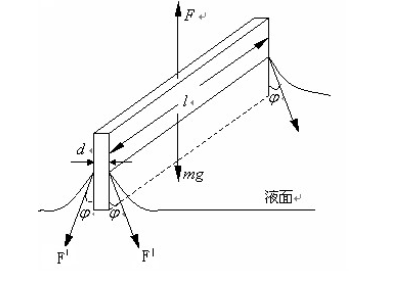
\includegraphics[scale=0.8]{原理图.png}
    \caption{实验原理}
\end{figure}
在金属丝框拉出水面的过程中,金属丝框在下面带起一水膜,当水膜恰好被拉断时,各力的平衡条件为:
\begin{equation}
    F=mg+2F'
\end{equation}
而\begin{equation}
    F'=\sigma l
\end{equation}
因此
\begin{equation}
    \sigma=\frac{F-mg}{2l}
\end{equation}
\subsection{实验装置}
焦利氏秤,砝码(0.5g-5g),钢板尺(或其他尺子,做完实验来改)
\subsection{实验内容/步骤}
\noindent
一.确定焦利氏秤上锥形弹簧的劲度系数
\begin{itemize}
    \item[] 
    (1) 组装焦利氏秤,依次安装弹簧,镜子,砝码盘.调节支架底座的螺丝使秤框竖直,
小镜子应正好位于玻璃管中间.\\
(2) 逐次在砝码盘内放入砝码,每次增量 0.5g 的砝码,从 0.5g~5g 范围内增加.每次操
作都要调节升降钮,做到三线合一,即玻璃圆筒上的刻线,小平面镜上的刻线,圆筒刻线在平面镜中的像对齐.
记录升降杆的位置读数,计算出弹簧的劲度系数.
\end{itemize}
二.用金属圈测量自来水的表面张力系数:
\begin{itemize}
    \item[] 
    (1) 测量金属圈的直径 d;\\
(2) 取下砝码,在砝码盘下挂上金属圈,保持三线合一,记下此时升降杆读数;\\
(3) 将盛有自来水的烧杯放在焦利氏秤台上,调节平台的微调螺丝和升降钮,使金属圈浸入水面以下;\\
(4) 缓慢地旋转平台微调螺丝和升降钮,注意烧杯下降和金属杆上升时,始终保持三线合一,
当液膜刚要破裂时,记下金属杆的读数.测量 5 次,取平均,计算自来水的表面张力系数,并计算不确定度.
\end{itemize}
三.用金属丝测量肥皂水的表面张力系数:
\begin{itemize}
    \item[] 
    (1) 测量金属丝两脚之间的距离 s;\\
    (2) 重复上述二中的步骤(2)-(4),计算肥皂水的表面张力系数.
\end{itemize}
四.用二中的方法,测量并计算自配洗洁精溶液的表面张力系数,并得出关系曲线.
\section{数据记录与处理}
\section{思考与讨论}
\end{document}